\chapter{Background}\label{chap:Background}

\begin{Listing}[t]
\centering
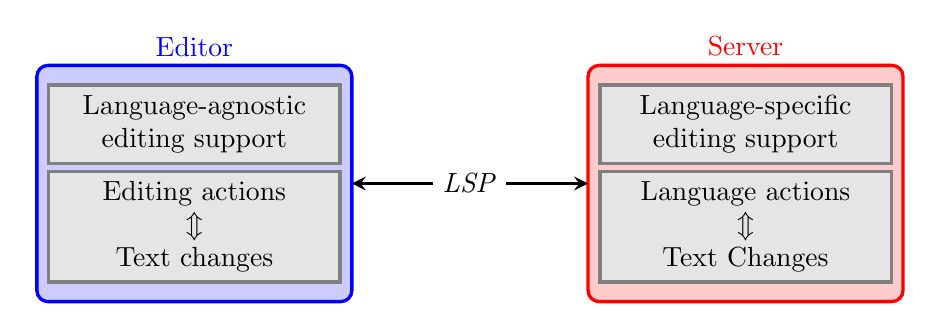
\begin{tikzpicture}
\draw[blue, very thick, rounded corners, fill=blue!20, anchor=north]
        (0,0) rectangle (4,3)
        node[anchor=north, align=center] at (2,3.5) {Editor};
\draw[gray, very thick, fill=gray!20]
        (0.15, 1.75) rectangle (3.85,2.75)
        node[black, text width=4cm, pos=.5, align=center] {Language-agnostic \linebreak editing support};
\draw[gray, very thick, fill=gray!20]
        (0.15, 0.25) rectangle (3.85,1.65)
        node[black, text width=4cm, pos=.5, align=center] {Editing actions \linebreak $\Updownarrow$ \linebreak  Text changes};

\draw[red, very thick, rounded corners, fill=red!20, anchor=north]
        (7,0) rectangle (11,3)
        node[anchor=north, align=center] at (9,3.5) {Server};
\draw[gray, very thick, fill=gray!20]
        (7.15, 1.75) rectangle (10.85,2.75)
        node[black, text width=4cm, pos=.5, align=center] {Language-specific \linebreak editing support};
\draw[gray, very thick, fill=gray!20]
        (7.15, 0.25) rectangle (10.85,1.65)
        node[black, text width=4cm, pos=.5, align=center] {Language actions \linebreak $\Updownarrow$ \linebreak Text Changes};

\draw[<->, very thick, >=stealth] (4,1.5) -- (7,1.5)
        node[midway,fill=white] {\emph{LSP}};
\end{tikzpicture}
\caption{LSP approach to language support. Borrowed from \cite{Rodriguez-Echeverria18a}}
\label{lst:lsp}
\end{Listing}

In this chapter, we provide an overview of the concepts and technologies that are relevant to the work presented in this thesis. We start by introducing the concept of language servers and the Language Server Protocol (LSP) in Section~\ref{sec:LanguageServerProtocol}. We then discuss language workbenches in Section~\ref{sec:LanguageWorkbenches}, type systems in Section~\ref{sec:TypeSystems}, and software and language product lines in Section~\ref{sec:SoftwareProductLines}.

The goal of this chapter is to provide the reader with the necessary background knowledge to understand the work presented in the following chapters. We assume that the reader has a basic understanding of programming languages and software development.

\section{Language Server Protocol}\label{sec:LanguageServerProtocol}
The Language Server Protocol\footnote{\url{https://microsoft.github.io/language-server-protocol}} (LSP) is a protocol that allows for the communication between a language server and an editor or an IDE. The LSP is used to decuple the a language-agnotic editor or integrated development environment (IDE) from the language-specific features of a language server (see Listing~\ref{lst:lsp}). This allows for the development of language servers that can be used with multiple editors or IDEs. The LSP is based on the stateless JSON-RPC protocol and defines a set of messages that are used to communicate between the language server and the editor or IDE.

Usually, the LSP Clients are developed as plugins for popular editors or IDEs decresing the effort to support a new language in a given editor. The LSP Clients are responsible for sending requests to the language server and processing the responses. The language server is responsible for providing language-specific features. The LSP defines a set of messages that are used to communicate between the language server and the editor or IDE. These messages include requests for code completion, code navigation, and code analysis, as well as notifications for changes to the document, diagnostics, and progress reports.

Language servers are \textit{de facto} standard for providing language-specific features in editors and IDEs. The LSP is supported by a wide range of editors and IDEs, including Noevim\footnote{\url{https://neovim.io/doc/user/lsp.html}}, Visual Studio Code\footnote{\url{https://code.visualstudio.com/api/language-extensions/language-server-extension-guide}}, Eclipse\footnote{\url{https://www.eclipse.org/community/eclipse_newsletter/2017/may/article1.php}}, and IntelliJ IDEA\footnote{\url{https://plugins.jetbrains.com/docs/intellij/language-server-protocol.html}}. There are several language servers available for popular programming languages, including Rust, TypeScript, Python, and Java and most of them are open-source\footnote{\url{https://microsoft.github.io/language-server-protocol/implementors/servers}}.

The LSP is initiated by Microsoft and is now an open standard that is maintained by the Language Server Protocol Working Group. It was designed for the use with the Visual Studio Code editor, but it has since been adopted by other editors and IDEs. The LSP is under open-source license and is available on GitHub\footnote{\url{https://github.com/microsoft/language-server-protocol}}.

\subsection{JSON-RPC}\label{subsec:JSONRPC}
The LSP uses JSON-RPC to communicate between a language server and an editor. JSON-RPC (v2)\footnote{\url{https://www.jsonrpc.org/specification}} is a stateless, light-weight remote procedure call (RPC) \cite{Birrell84} protocol that uses JSON as the data format.

RPC is a protocol that allows a client to call a procedure on a remote server. The client sends a request to the server, and the server sends a response back to the client. The JSON-RPC protocol defines a set of messages that are used to communicate between the client and the server. These messages include requests, responses, and notifications. The JSON-RPC protocol is designed to be simple and easy to implement, making it well-suited for use in web applications and other distributed systems.

JSON-RPC is a JSON based implementation of the RPC protocol. It defines a set of rules for encoding and decoding JSON data, as well as a set of rules for \textit{Request}, \textit{Notification}, and \textit{Response} messages. The messages are sent over a transport layer, such as HTTP or WebSockets. The JSON-RPC protocol is designed to be simple and easy to implement, making it well-suited for use in web applications and other distributed systems.

All messages refer to a \textit{method} that is a string containing the name of the method to be called. The \textit{params} field is an array or object containing the parameters to be passed to the method. Typically, messages are synchronous, meaning that the client waits for a response from the server before continuing. The \textit{id} field is a unique identifier for the message, which is used to match requests with responses. However, the JSON-RPC protocol also supports asynchronous messages, known as notifications, which do not require a response from the server. This is implemented by setting the \textit{id} field to \textit{null}, in which case the server does not send a response back to the client.

The JSON-RPC specification includes the ability for clients to batch multiple requests or notifications by sending them as a list. The server is expected to respond with a corresponding list of results for each request. Additionally, the server has the flexibility to process these requests concurrently.

\subsection{Command Specifications}\label{sec:CommandSpecification}
The LSP is defined on top of the JSON-RPC protocol described in section \ref{subsec:JSONRPC}. In abstract terms, the LSP defines a set of command that can be sent between a client and a server. In the Language Server Protocol Specification\footnote{https://microsoft.github.io/language-server-protocol/specifications/lsp/3.17/specification}, these commands are divided into four categories: \textit{Language Features}, \textit{Text Document Synchronization}, \textit{Workspace Features}, and \textit{Window Features}.

\subsubsection{Language Features}\label{subsec:LanguageFeatures}
The \textit{Language Features} provide the smarts of the language server. Usually, the client sends a request to the server to get information about the document as a tuple of \texttt{TextDocument} and \texttt{Position}. \textit{Code comprehension} and \textit{Coding Features} are the two main categories of commands in this category.

Here a brief description of the most important commands in this category:
\begin{itemize}
    \item \texttt{textDocument/completion}: The completion request is sent from the client to the server to compute completion items at a given cursor position. Completion items are presented in the editor's user interface. If computing full completion items is expensive, servers can additionally provide a handler for the completion item resolve request (\texttt{completionItem/resolve}). This request is sent when a completion item is selected in the user interface.
    \item \texttt{textDocument/hover}: The hover request is sent from the client to the server to request hover information at a given text document position. Hover information typically includes the symbol's signature and documentation.
    \item \texttt{textDocument/definition}: The definition request is sent from the client to the server to resolve the definition location of a symbol at a given text document position.
    \item \texttt{textDocument/references}: The references request is sent from the client to the server to resolve project-wide references for the symbol denoted by the given text document position.
    \item \texttt{textDocument/documentHighlight}: The document highlight request is sent from the client to the server to resolve a document highlights for a given text document position. For programming languages, this usually highlights all references to the symbol denoted by the given text document position.
\end{itemize}

\subsubsection{Text Document Synchronization}\label{subsec:TextDocumentSynchronization}
The \textit{Text Document Synchronization} commands are used to notify the server of changes to the document. Client support for \texttt{textDocument/didOpen}, \texttt{textDocument/didChange}, \texttt{textDocument/didClose} is mandatory. This includes the ability to fully and incrementally synchronize changes to the document, such as inserting, deleting, and replacing text.

Here a brief description of the most important commands in this category:
\begin{itemize}
    \item \texttt{textDocument/didOpen}: The document open notification signals that the client is now managing a text document. The server should not read the document using its URI. Open notifications are balanced with close notifications, with only one open notification allowed at a time for a document. The server's ability to fulfill requests is unaffected by a document's open or closed status.
    \item \texttt{textDocument/didChange}: The document change notification is sent from the client to the server to signal changes to a text document. In response, the server should compute a new version of the document's content. The server should not rely on the client to send a specific sequence of change events. The server is free to compute the new version of the document on the fly.
    \item \texttt{textDocument/didClose}: The document close notification is sent from the client to the server when the document is no longer managed by the client. The document's URI is no longer valid and the server should not resolve the document using the URI.
    \item \texttt{textDocument/didSave}: The document save notification is sent from the client to the server when the document is saved. The notification is sent after the document has been saved.
\end{itemize}

\subsubsection{Workspace Features}\label{subsec:WorkspaceFeatures}
The \texttt{Workspace Features} category includes commands that allow the client to interact with the workspace. The workspace is the collection of open documents and the client's configuration. The workspace commands are used to manage the workspace, such as symbol search, workspace configuration and client configuration.

Here a brief description of the most important commands in this category:
\begin{itemize}
    \item \texttt{workspace/symbol}: The workspace symbol request is sent from the client to the server to list project-wide symbols matching the query string. The request can be used to populate a list of symbols matching the query string in the user interface.
    \item \texttt{workspace/configuration}: The workspace configuration request is sent from the client to the server to fetch configuration settings from the server. The request can fetch configuration settings from the client's workspace or from the server's configuration.
    \item \texttt{workspace/didChangeConfiguration}: The configuration change notification is sent from the client to the server to signal changes to the client's configuration settings. The server should use the new configuration settings to update its behavior.
    \item \texttt{workspace/didChangeWorkspaceFolders}: The workspace folder change notification is sent from the client to the server to signal changes to the workspace's folders. The server should use the new workspace folders to update its behavior.
\end{itemize}

\subsubsection{Window Features}\label{subsec:WindowFeatures}

The \texttt{Window Features} category includes commands that allow the client to interact with the window. The window is the client's user interface, such as the editor, the sidebar, and the status bar. The window commands are used to manage the window, such as showing messages, showing notifications, and showing progress.

Here a brief description of the most important commands in this category:
\begin{itemize}
    \item \texttt{window/showMessage}: The show message notification is sent from the server to the client to show a message to the user. The message can be shown in a variety of ways, such as a dialog box, a status bar, or a notification.
    \item \texttt{window/showMessageRequest}: The show message request is sent from the server to the client to show a message to the user and get a response. The message can be shown in a variety of ways, such as a dialog box, a status bar, or a notification.
    \item \texttt{window/logMessage}: The log message notification is sent from the server to the client to log a message. The message can be logged in a variety of ways, such as a console, a file, or a database.
    \item \texttt{window/showMessageRequest}: The show message request is sent from the server to the client to show a message to the user and get a response. The message can be shown in a variety of ways, such as a dialog box, a status bar, or a notification.
\end{itemize}

\subsection{Key Methods Overview}\label{subsec:KeyMethodsOverview}

Six \textit{key methods} have been identified by langserver organization\footnote{\url{https://langserver.org}} as the most important methods to be implemented by a language server. These capabilities are:
\begin{enumerate}
    \item \textbf{Diagnostic Analyze} source code --- Parse and Type-check the source code to provide diagnostics.
    \item \textbf{Workspace/Document Symbols} --- List all symbols in the workspace.
    \item \textbf{Jump to Definition} --- Find and jump to the definition of a symbol.
    \item \textbf{Find References} --- List all usages of a symbol.
    \item \textbf{Hover Information} --- Show information about a symbol at the cursor.
    \item \textbf{Code Completion} --- Provide completions for a symbol at the cursor.
\end{enumerate}

\subsubsection{Diagnostic Analysis}\label{subsubsec:DiagnosticAnalysis}

The diagnostic analysis is the process of parsing and type-checking the source code to provide diagnostics. The diagnostics are used to identify errors and warnings in the source code, such as syntax errors, type errors, and unused variables. The diagnostics are presented to the user in the editor's user interface, such as a list of errors and warnings in the sidebar.

File update and diagnostic analysis are passive. Thay are sent as notifications in order to avoid blocking communication between the client and the server.

In the figure \ref{fig:diagnostic} we can see an example of diagnostics in Neovim generated by the Rust Language Server. It shows a list of errors and suggestions coused by the concatenation of two \texttt{\&str} variables.

\begin{figure}[t]
    \centering
    \fcolorbox{black}{white}{
        \includegraphics[width=0.9\linewidth]{imgs/background_diagnostic.png}
    }
    \caption{Showing diagnostics in Neovim generated by the Rust Language Server.}
    \label{fig:diagnostic}
\end{figure}

\subsubsection{Workspace/Document Symbols}\label{subsubsec:WorkspaceDocumentSymbols}

\fbox{
    \parbox{\textwidth}{
        \centering
        \textbf{RPC Method}:  \href{https://microsoft.github.io/language-server-protocol/specifications/lsp/3.17/specification/\#workspace_symbol}{textDocument/workspaceSymbol} or \href{https://microsoft.github.io/language-server-protocol/specifications/lsp/3.17/specification/\#textDocument_documentSymbol}{textDocument/documentSymbol}
    }
}
\hfill \break

\noindent
This feature is defined as both a \textit{Language Feature} and \textit{Workspace Feature}.

The \texttt{textDocument/workspaceSymbol} request is sent from the client to the server to list project-wide symbols matching the query string. The request can be used to populate a list of symbols matching the query string in the user interface. The granularity of the listed symbols depends on the language server implementation.

The difference between \texttt{textDocument/workspaceSymbol} and \texttt{textDocument/documentSymbol} is that the first one takes into account the visibility of the symbols in the workspace showing only the public ones. The second one shows all symbols in the document.


\subsubsection{Jump to Definition}\label{subsubsec:JumpToDefinition}
\fbox{
    \parbox{\textwidth}{
        \centering
        \textbf{RPC Method}:  \href{https://microsoft.github.io/language-server-protocol/specifications/lsp/3.17/specification/\#textDocument_definition}{textDocument/definition}
    }
}
\hfill \break

The code navigation is an important feature of the LSP.

The \texttt{textDocument/definition} request is sent from the client to the server to resolve the definition location of a symbol at a given text document position. The server should return the location of the symbol's definition, such as the file path and line number.

In the figure \ref{fig:hover} we can see that at the top of floating window there is the signature of the function \texttt{hello\_world} meaning that the goind to definition will take us to the function definition.

\subsubsection{Find References}
\fbox{
    \parbox{\textwidth}{
        \centering
        \textbf{RPC Method}:  \href{https://microsoft.github.io/language-server-protocol/specifications/lsp/3.17/specification/\#textDocument_references}{textDocument/references}
    }
}
\hfill \break

The retrieval of references is the inverse of the jump to definition explained in the previous section (\ref{subsubsec:JumpToDefinition}).

The \texttt{textDocument/references} request is sent from the client to the server to resolve project-wide references for the symbol denoted by the given text document position. The server should return a list of references to the symbol, such as the file path, line number, and the column number.

In the figure \ref{fig:references} we can see that the function \texttt{hello\_world} is being referenced twice in the \texttt{main} function and another occurence is the function definition. In fact, three references are shown in the right window.

\begin{figure}[t]
    \centering
    \fcolorbox{black}{white}{
        \includegraphics[width=0.9\linewidth]{imgs/background_references.png}
    }
    \caption{Finding references in Neovim generated by the Rust Language Server.}
    \label{fig:references}
\end{figure}

\subsubsection{Hover Information}

\fbox{
    \parbox{\textwidth}{
        \centering
        \textbf{RPC Method}:  \href{https://microsoft.github.io/language-server-protocol/specifications/lsp/3.17/specification/\#textDocument_hover}{textDocument/hover}
    }
}
\hfill \break

The hover information is a feature that shows information about a symbol at the cursor. The information typically includes the symbol's signature and documentation. This is triggered by the user hovering the mouse over a symbol in the editor or by pressing a keybinding.

A request is sent from the client to the server to request hover information at a given text document position. The server should return hover information for the symbol at the given position, such as the symbol's signature and documentation.

In the figure \ref{fig:hover} we can see that the function \texttt{hello\_world} is being hovered and the signature of the function is shown in the floating window. The signature is \texttt{fn hello\_world() -> String} and the documentation, written in the comment above the function, is also shown.

\begin{figure}[t]
    \centering
    \fcolorbox{black}{white}{
        \includegraphics[width=0.9\linewidth]{imgs/background_hover.png}
    }
    \caption{Hover information in Neovim generated by the Rust Language Server.}
    \label{fig:hover}
\end{figure}

\subsubsection{Code Completion}
\fbox{
    \parbox{\textwidth}{
        \centering
        \textbf{RPC Method}:  \href{https://microsoft.github.io/language-server-protocol/specifications/lsp/3.17/specification/\#textDocument_completion}{textDocument/completion}
    }
}
\hfill \break

The code completion is a feature that provides completions for a symbol at the cursor. The completions are presented in the editor's user interface. If computing full completion items is expensive, servers can additionally provide a handler for the completion item resolve request (\texttt{completionItem/resolve}). This request is sent when a completion item is selected in the user interface.

Usually, the completion is triggered by the user typing a character or pressing a keybinding in proximity to a character, such as \texttt{.}, \texttt{::}, or \texttt{->}.

In the figure \ref{fig:completion} we can see that the code completion is triggered by the user typing \texttt{to\_} and pressing \texttt{<C-n>} in the editor. Two float windows are shown with the completion items. The first one shows the options for the \texttt{to\_} function associated with the \texttt{\&str} type and the second one shows the documentation of the selected completion item.

\begin{figure}[h]
    \centering
    \fcolorbox{black}{white}{
        \includegraphics[width=0.9\linewidth]{imgs/background_completion.png}
    }
    \caption{Code completion in Neovim generated by the Rust Language Server.}
    \label{fig:completion}
\end{figure}


\section{Language Workbenches}\label{sec:LanguageWorkbenches}

\section{Type Systems}\label{sec:TypeSystems}

\section{Software and Language Product Lines}\label{sec:SoftwareProductLines}
